% Created 2021-07-13 Tue 15:28
% Intended LaTeX compiler: pdflatex
\documentclass[11pt]{article}
\usepackage[utf8]{inputenc}
\usepackage[T1]{fontenc}
\usepackage{graphicx}
\usepackage{grffile}
\usepackage{longtable}
\usepackage{wrapfig}
\usepackage{rotating}
\usepackage[normalem]{ulem}
\usepackage{amsmath}
\usepackage{textcomp}
\usepackage{amssymb}
\usepackage{capt-of}
\usepackage{hyperref}
\date{\today}
\title{}
\hypersetup{
 pdfauthor={},
 pdftitle={},
 pdfkeywords={},
 pdfsubject={},
 pdfcreator={Emacs 27.2 (Org mode 9.4.6)}, 
 pdflang={English}}
\begin{document}

\tableofcontents

\section{Discussão}
\label{sec:org2914655}

Pelas Tabelas 3 (valor de \(k\) das amostras), e a tabela experimental dado no roteiro do relatório \footnote{Encontrada em https://edisciplinas.usp.br/pluginfile.php/6266829/mod_resource/content/0/roteiro.pdf},

\begin{center}
\begin{tabular}{lll}
\hline
Amostras & \(R_{esp}\) (\$\(\Omega\)\$/m) & k\textsubscript{REF} (W/mK)\\
\hline
Fibra de vidro & 2,356(8) & 0,04 a 0,05[4]\\
Teflon & 17,75(3) & 0,250[4]\\
Argamassa & 38,01(5) & 0,6 a 1,6[5]\\
Stycast + 10\% AlN & 15,98(4) & 0,320(4)[2]\\
\hline
\end{tabular}
\end{center}
Reproduçao  da tabela do roteiro experimental, original em: \cite{rebeca2021}

Os valores de Fibra de vidro e Stycast + 10\% AlN (Resina) se encontram fora do intervalo de confiança derivado dos dados experimentais. O Teflon e a Argamassa estão de acordo com a literatura.

\subsection{Fontes de erro}
\label{sec:orgf9934ec}
\subsubsection{Fibra de vidro}
\label{sec:org8c14fd0}
É possível se observar pela, Figura 5 Temperatura vs Int(t) - Fibra de Vidro, que os valores medidos destoam em sua temperatura de medição de quase dez graus celcius. Assim, o valor encontrado de 0,071(3), por mais que próximo do intervalo de 0,04 e 0,05, foi feita a temperaturas entre 33 e 49 celcius. O que nos leva a entender que a medida está enviesada superiormente \cite{ochs2005temperature,budaiwi2002variations}, como foi observado.

O efeito pode também ser explicado pela lei de Wiedemman-Franz (\autoref{eq:WF}). Pois, a condutividade em isolantes aumenta com a temperatura, por causa dos phonos, assim, k deve aumentar também, para que a relação se satisfaça.

\href{k-var.png}{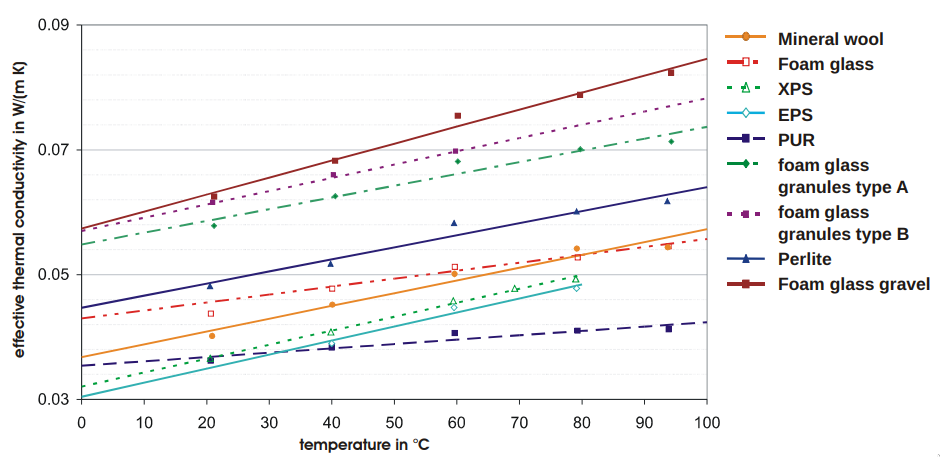
\includegraphics[width=.9\linewidth]{/home/buddhilw/PP/Faculdade/MEFIII/exp6/k-var.png}}
Fonte: \cite{ochs2005temperature}

O trabalho "Temperature and Moisture Dependence of the Thermal Conductivity of Insulation Materials", nos tras gráficos de diversas variações de condutividade térmica, com isolantes, como a fibra de vidro. Vemos que a dependência é linear, e dez graus pode ser uma grande influência para alguns materiais, dependendo de seu \(\alpha\).

\begin{equation}
k_{eff} = k_0 + \alpha (T - 273.15)
\end{equation}


\begin{verbatim}
@article{ochs2005temperature,
title={Temperature and moisture dependence of the thermal conductivity of insulation materials},
author={Ochs, F and M{\"u}ller-Steinhagen, H},
journal={NATO Advanced Study Institute on Thermal Energy Storage for Sustainable Energy Consumption (TESSEC), Izmir, Cesme},
year={2005}}
\end{verbatim}

\begin{verbatim}
@article{budaiwi2002variations,
  title={Variations of thermal conductivity of insulation materials under different operating temperatures: Impact on envelope-induced cooling load},
  author={Budaiwi, I and Abdou, A and Al-Homoud, M},
  journal={Journal of architectural engineering},
  volume={8},
  number={4},
  pages={125--132},
  year={2002},
  publisher={American Society of Civil Engineers}
}
\end{verbatim}

\begin{verbatim}
@misc{rebeca2021,
 title={Condutividade térmica via m\'etodo do fio quentem, Roteiro e Guia},
 author={Rebeca Bacani},
 journal={Escola de Engenharia de Lorena - Universidade de São Paulo (USP)},
 year={2021}}
\end{verbatim}

\subsubsection{Resina}
\label{sec:org2e67173}
O erro experimental da resina pode ser explicado igualmente, com base na diferença de temperatura iniais das medidas.

Ademais,
\begin{quote}
The thermal conductivity of the epoxy matrix has the shape which is characteristic of that of amorphous glasses and polymers. The conductivity increases monotonically with temperature apart from the plateau
region around 10 K \cite{garrett1974thermal}.
\end{quote}

A epoxy possui acentuadas diferenças de valores de \(k\), dado a concentração do material que a preenche e a condutividade desse material interno. O valores de compósitos sendo maiores do que os da resina pura. Quando se aumenta o material preenchido, maior é seu valores de condutividade térmica.

\begin{quote}
The value at a given temperature is in general dependent on the volume concentration of the filler and on its thermal conductivity. 

In all the samples the composite conductivity above 20 K is higher than that of the unfilled resin and it increases with increasing filler concentration. \cite{garrett1974thermal}.
\end{quote}

Assim, o valor de 10\% de AlN pode ter influenciado consideravelmente o valor de \(k\).

\begin{verbatim}
@article{garrett1974thermal,
  title={The thermal conductivity of epoxy-resin/powder composite materials},
  author={Garrett, KW and Rosenberg, HM},
  journal={Journal of Physics D: Applied Physics},
  volume={7},
  number={9},
  pages={1247},
  year={1974},
  publisher={IOP Publishing}}
\end{verbatim}
\end{document}